\section{Ponteiros}


\subsection{}
\subsubsection*{Código}
\lstinputlisting{q1_l1.c}
\subsubsection*{Saída}
\begin{figure}[h!]
	\centering
	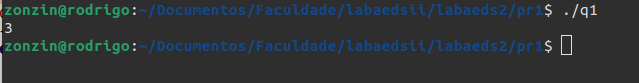
\includegraphics[width=0.7\linewidth]{imagens/screenshot001}
	\caption{Q1}
	\label{fig:screenshot001}
\end{figure}

\newpage
\subsection{}
\subsubsection*{Código}
\textbf{ATENÇÃO: para a execução correta desse código é necessário passar o tamanho desejado  $n$  como argumento da main.}

\textbf{./q2 10}

\begin{multicols}{2}
	\lstinputlisting{q2_l1.c}
\end{multicols}
\subsubsection*{Saída}
\begin{figure}[h!]
	\centering
	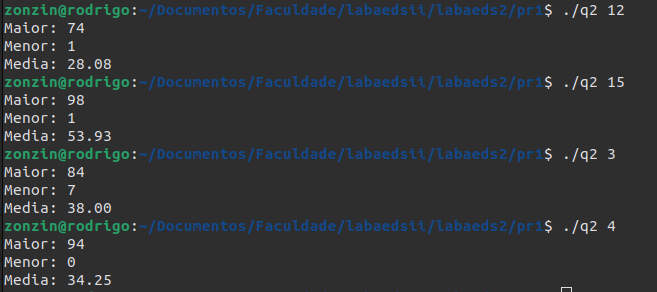
\includegraphics[width=0.7\linewidth]{imagens/saida_q2}
	\caption{Q2}
	\label{fig:saidaq2}
\end{figure}

\newpage

\subsection{}
\subsubsection*{Código}
\begin{multicols}{2}
	\lstinputlisting{q3_l1.c}
\end{multicols}
\subsubsection*{Saída}
\begin{figure}[h!]
	\centering
	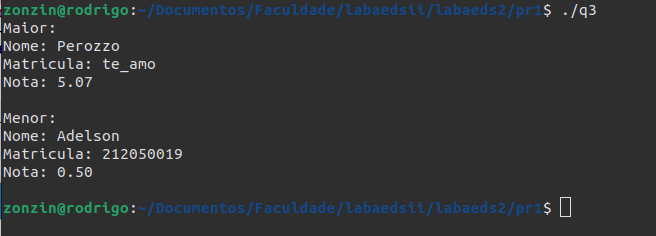
\includegraphics[width=0.5\linewidth]{imagens/saida_q3}
	\caption{Q3}
	\label{fig:saidaq3}
\end{figure}

\newpage

\subsection{}
\subsubsection*{Código}
\textbf{ATENÇÃO: passe os valores $a$, $b$, e $c$ como parâmetro da main.}

Por exemplo, para calcularmos $x^2+x-12=0$, usamos:

\textbf{./q4 1 1 -12}
\begin{multicols}{2}
	\lstinputlisting{q4_l1.c}
\end{multicols}

\subsubsection*{Saída}
\begin{figure}[h!]
	\centering
	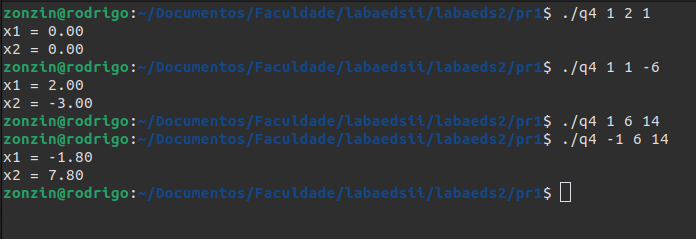
\includegraphics[width=0.7\linewidth]{imagens/saida_q4}
	\caption{Q4}
	\label{fig:saidaq4}
\end{figure}


\newpage
\section{Recursividade}

\subsection{}
\subsubsection*{Código}
\textbf{ATENÇÃO: } passar $n=5$ como parâmetro no terminal. 
\lstinputlisting{q5_l1.c}
\subsubsection*{Saída}
\begin{figure}[h!]
	\centering
	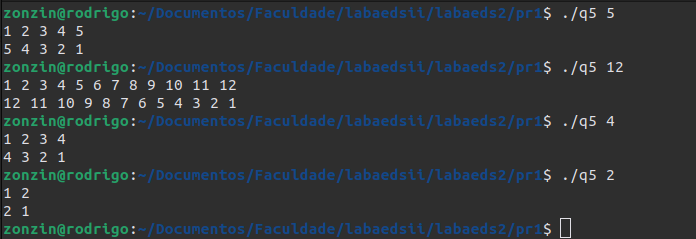
\includegraphics[width=0.7\linewidth]{imagens/saida_q5}
	\caption{Para uma entrada de $n = 5$ no terminal}
	\label{fig:saidaq5}
\end{figure}


\subsection{}
\subsubsection*{Código}
\lstinputlisting{q6_l1.c}
\subsubsection*{Saída}
\begin{figure}[h!]
	\centering
	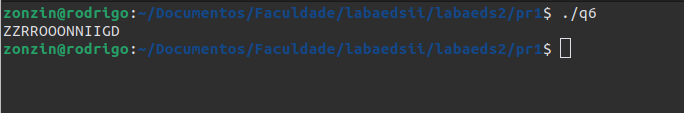
\includegraphics[width=0.7\linewidth]{imagens/saida_q6}
	\caption{Saída para a string "RODRIGOZONZIN"}
	\label{fig:saidaq6}
\end{figure}

\newpage
\subsection{}
\textbf{ATENÇÃO:} A implementação desse código é mais sutil. Seja a sequência natural $S = 3, 4, 5, 6, 7$ . 
A recursividade deve partir do elemento $S_n$ (o mais externo) até o elemento $S_1$ (o primeiro), da seguinte forma: 
$$ 3 + 4 + 5 + 6 + 7 $$
$$ 3 + 4 + 5 + 6  $$
$$ 3 + 4 + 5  $$
$$ 3 + 4 $$

Para fazermos a soma de uma sequência de elementos naturais em um intervalo $[k, n]$ qualquer, nos valemos da seguinte propriedade: 

$$ \sum_{i =k }^{n} = \sum_{i=1}^{n} - \sum_{i=1}^{k-1}$$


Dessa maneira, operamos a soma gaussiana sobre todos os subintervalos até que a diferença de um intervalo $[k_i, n_i] : n_i - k_1 \leq 0$, \textit{i. e.}, a condição de parada foi atingida. 

\subsubsection*{Código}
\lstinputlisting{q7_l1.c}
\subsubsection*{Saída}
\begin{figure}[h!]
	\centering
	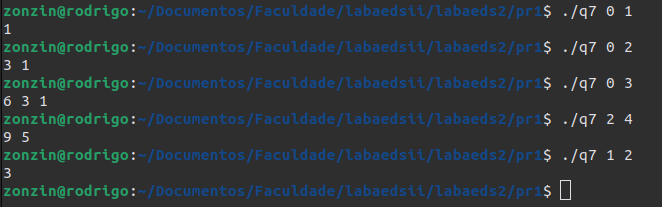
\includegraphics[width=0.7\linewidth]{imagens/saida_q7}
	\caption{Resultado para várias saídas}
	\label{fig:saidaq7}
\end{figure}

\newpage
\subsection{}
A implementação é trivial.
\subsubsection*{Código}
\lstinputlisting{q8_l1.c}
\subsubsection*{Saída}

\subsection{}
Utilizamos a \textit{flag} -555 para preencher o valor recursivamente. 
\subsubsection*{Código}
\begin{multicols}{2}
	\lstinputlisting{q9.c}
\end{multicols}

\subsubsection*{Saída}
\begin{figure}[h!]
	\centering
	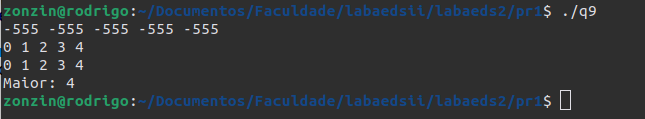
\includegraphics[width=0.7\linewidth]{imagens/saida_q9}
	\caption{Q9}
	\label{fig:saidaq9}
\end{figure}

\subsection{}
O código foi analisado, executado e entendido para 1, 2, 3, 4 e 5 discos.

